\section{Robustness of a BNN}

In the preceding section, a foundational approach was introduced for the robustness assessment of standard NNs, and this approach was extended to include additional aspects. The goal now is to apply this method to evaluate the robustness of BNNs.

In particular, the idea is to use the concepts introduced in \Chap~\ref{chap:c3} to compute the robustness of a BNN. The aim is to determine whether the incorporation of uncertainty, a characteristic of BNNs, renders them more robust than standard NNs. This evaluation will shed light on the comparative robustness of these two network architectures.

The use of classification with uncertainty yields two key metrics: accuracy and the unknown ratio. The approach presented in \Def~\ref{def:rob3} can still be applicable. From the measured accuracy, it is possible to apply the same formula to calculate the robustness metric. The advantage of using the same definition is the comparability of the computed metrics between standard NNs and BNNs. This comparability is important when making a choice between these two models.

However, BNNs introduce a new dimension, which is the presence of unknown values, and this aspect is not currently considered when computing robustness. In fact, in cases where the network predicts only unknown values, the accuracy could still be $100\%$. The robustness formula would yield an output of $1$, but the network is essentially useless. Hence, there is a need to define a method that can account for this new aspect and provide a more comprehensive assessment of model quality.

One way to address this issue is to calculate a robustness metric using the same approach, but instead of using accuracy, the unknown ratio will be employed. This metric can be referred to as robustness against \textit{indecision}. This approach allows for the evaluation of the model robustness when it is uncertain or indecisive in its predictions, providing a more comprehensive assessment of its performance.

\begin{definition}\label{def:robind} (Indecision robustness).
	Let $C$ be a classifier, $tol(x)$ a tolerance function and $dep(x)$ a penalization function.
	The robustness against indecision $robInd_A(C,D) \in [0,1]$ of a classifier $C$ w.r.t. alteration of type A in the range $[L_A, U_A]$ on a dataset $D$ is defined formally as:
	\[
		robInd_A(C,D) = \frac{\int_{L_A}^{U_A} [tol(\gamma - ind(C,D^{A_i})) - dep(\gamma - ind(C,D^{A_i}))] \cdot p_A(i)\ di}{2} + \frac{1}{2}
	\]
	
	where $\gamma$ is a threshold referring to maximum unknown ratio accepted, $p_A$ is probability distribution of the alteration levels and $ind(C,D^{A_i})$ is the unknown ratio of $C$ evaluated on $D^{A_i}$.
\end{definition}

This metric quantifies the network resilience in terms of unknown predictions. It follows the same definition as robustness, enabling a direct comparison between the two metrics to comprehensively evaluate the network performance, particularly in situations where it exhibits indecision or uncertainty in its predictions.

\subsection{Effectiveness}

It is evident that the most important property is robustness since it considers accuracy, which is of primary importance in practical situations. Indecision, while informative about network quality, serves as a secondary metric for evaluation. However, a network with high accuracy and a significant proportion of unknown predictions is also not useful. This highlights the need to evaluate both of these metrics together in some way.

For this reason, a new measure will be introduced to combine both accuracy and the unknown ratio. This concept takes the name of \textit{effectiveness}. It describes how effective the network is in its predictions. In other words, it means that a network outputting only unknown values is as ineffective as one that produces solely incorrect predictions. To construct this metric, we need to reason about the desired behavior:

\begin{itemize}
	\item When the network has an unknown ratio equal to zero, the effectiveness should reflect the accuracy value;
	\item When there are unknown predictions, the effectiveness should be lower than the accuracy. Specifically, for a given accuracy value, the effectiveness should decrease as the unknown ratio increases.
\end{itemize}

These principles ensure that the effectiveness metric aligns with the accuracy while also accounting for the presence of unknown predictions.

Following this considerations, a suitable way to express the effectiveness is by using a ratio:
\[
	eff(C,D) = \frac{acc(C,D)}{ind(C,D) + 1}
\]

This score is directly proportional to accuracy and inversely proportional to the unknown ratio, with both quantities falling within the range of $[0,1]$. The addition of $1$ in the denominator prevents division by zero. This formulation reflects the desired behavior where effectiveness is influenced by accuracy but decreases as indecisiveness increases. 

To analyze the behavior of this metric, consider the following observations:
\begin{itemize}
	\item $eff(C,D)$ always assumes values in the range $[0,1]$, aligning with the desired range for such a metric.;
	\item When $ind(C,D)=0$ $eff(C,D) = acc(C,D)$ which was one of the desired behaviors;
	\item If $ind(C,D) \ne 0$, accuracy is divided by a number greater than 1, resulting in a lower score, which satisfies the second desired behavior;
	\item Furthermore, whenever the $acc(C,D) = 0$ the effectiveness is also zero. This is logical because if there are no good predictions (accuracy is zero), the network is essentially useless, aligning with practical expectations.
\end{itemize}

The proposed formula indeed serves as a suitable quality measure BNNs as it effectively combines the two key aspects: correct and unknown predictions.
However, there can be a scenario where $acc(C,D)=1$ and $ind(C,D)=1$, i.e., the network is exclusively predicting unknown values. This is a specific case where the network is essentially useless, and in such a scenario, the effectiveness should ideally be 0. With the above formula, it would be $eff(C,D)=0.5$.
To address this issue and ensure that effectiveness reflects this scenario, the idea is to multiply the ratio by $(1-ind(C,D))$. This adjustment would yield a more appropriate measure of effectiveness in situations where the network predominantly predicts unknown values.

\begin{definition} (Effectiveness).
	The effectiveness of a classifier $C$ on dataset $D$ is defined as:
	\[
		eff(C,D) = \frac{acc(C,D) \cdot (1 - ind(C,D))}{ind(C,D) + 1}
	\]
\end{definition}

\Fig~\ref{fig:eff_vs} illustrates graphically the behavior of this formula when one of the two variables is fixed. In particular \Fig~\ref{fig:eff_vs_acc} demonstrates that when $ind$ is fixed, effectiveness consists of a straight line. The slope of this line is determined by the unknown ratio. A higher $ind$ results in a lower slope, in other words the effectiveness is calculated by linearly interpolating between the highest achievable score, $\frac{1 - ind(C,D)}{ind(C,D) + 1}$, and $0$, the lowest score.

On the other side, \Fig~\ref{fig:eff_vs_ind}  illustrates the trend of effectiveness when accuracy is fixed. In this case, the behavior is different due to the presence of $ind(C,D)$ in the denominator.
This means that once accuracy is fixed, effectiveness decreases more steeply compared to a linear relationship. This behavior is actually desirable since it makes sense to weigh accuracy more than the unknown ratio. Specifically, for $ind$ values that are closer to the bounds, $eff$ varies more significantly. Additionally, accuracy sets the maximum achievable effectiveness score, and based on the unknown ratio, it can decrease from that point.

\begin{figure}[h]
	\centering
	\begin{subfigure}{.5\textwidth}
		\centering
		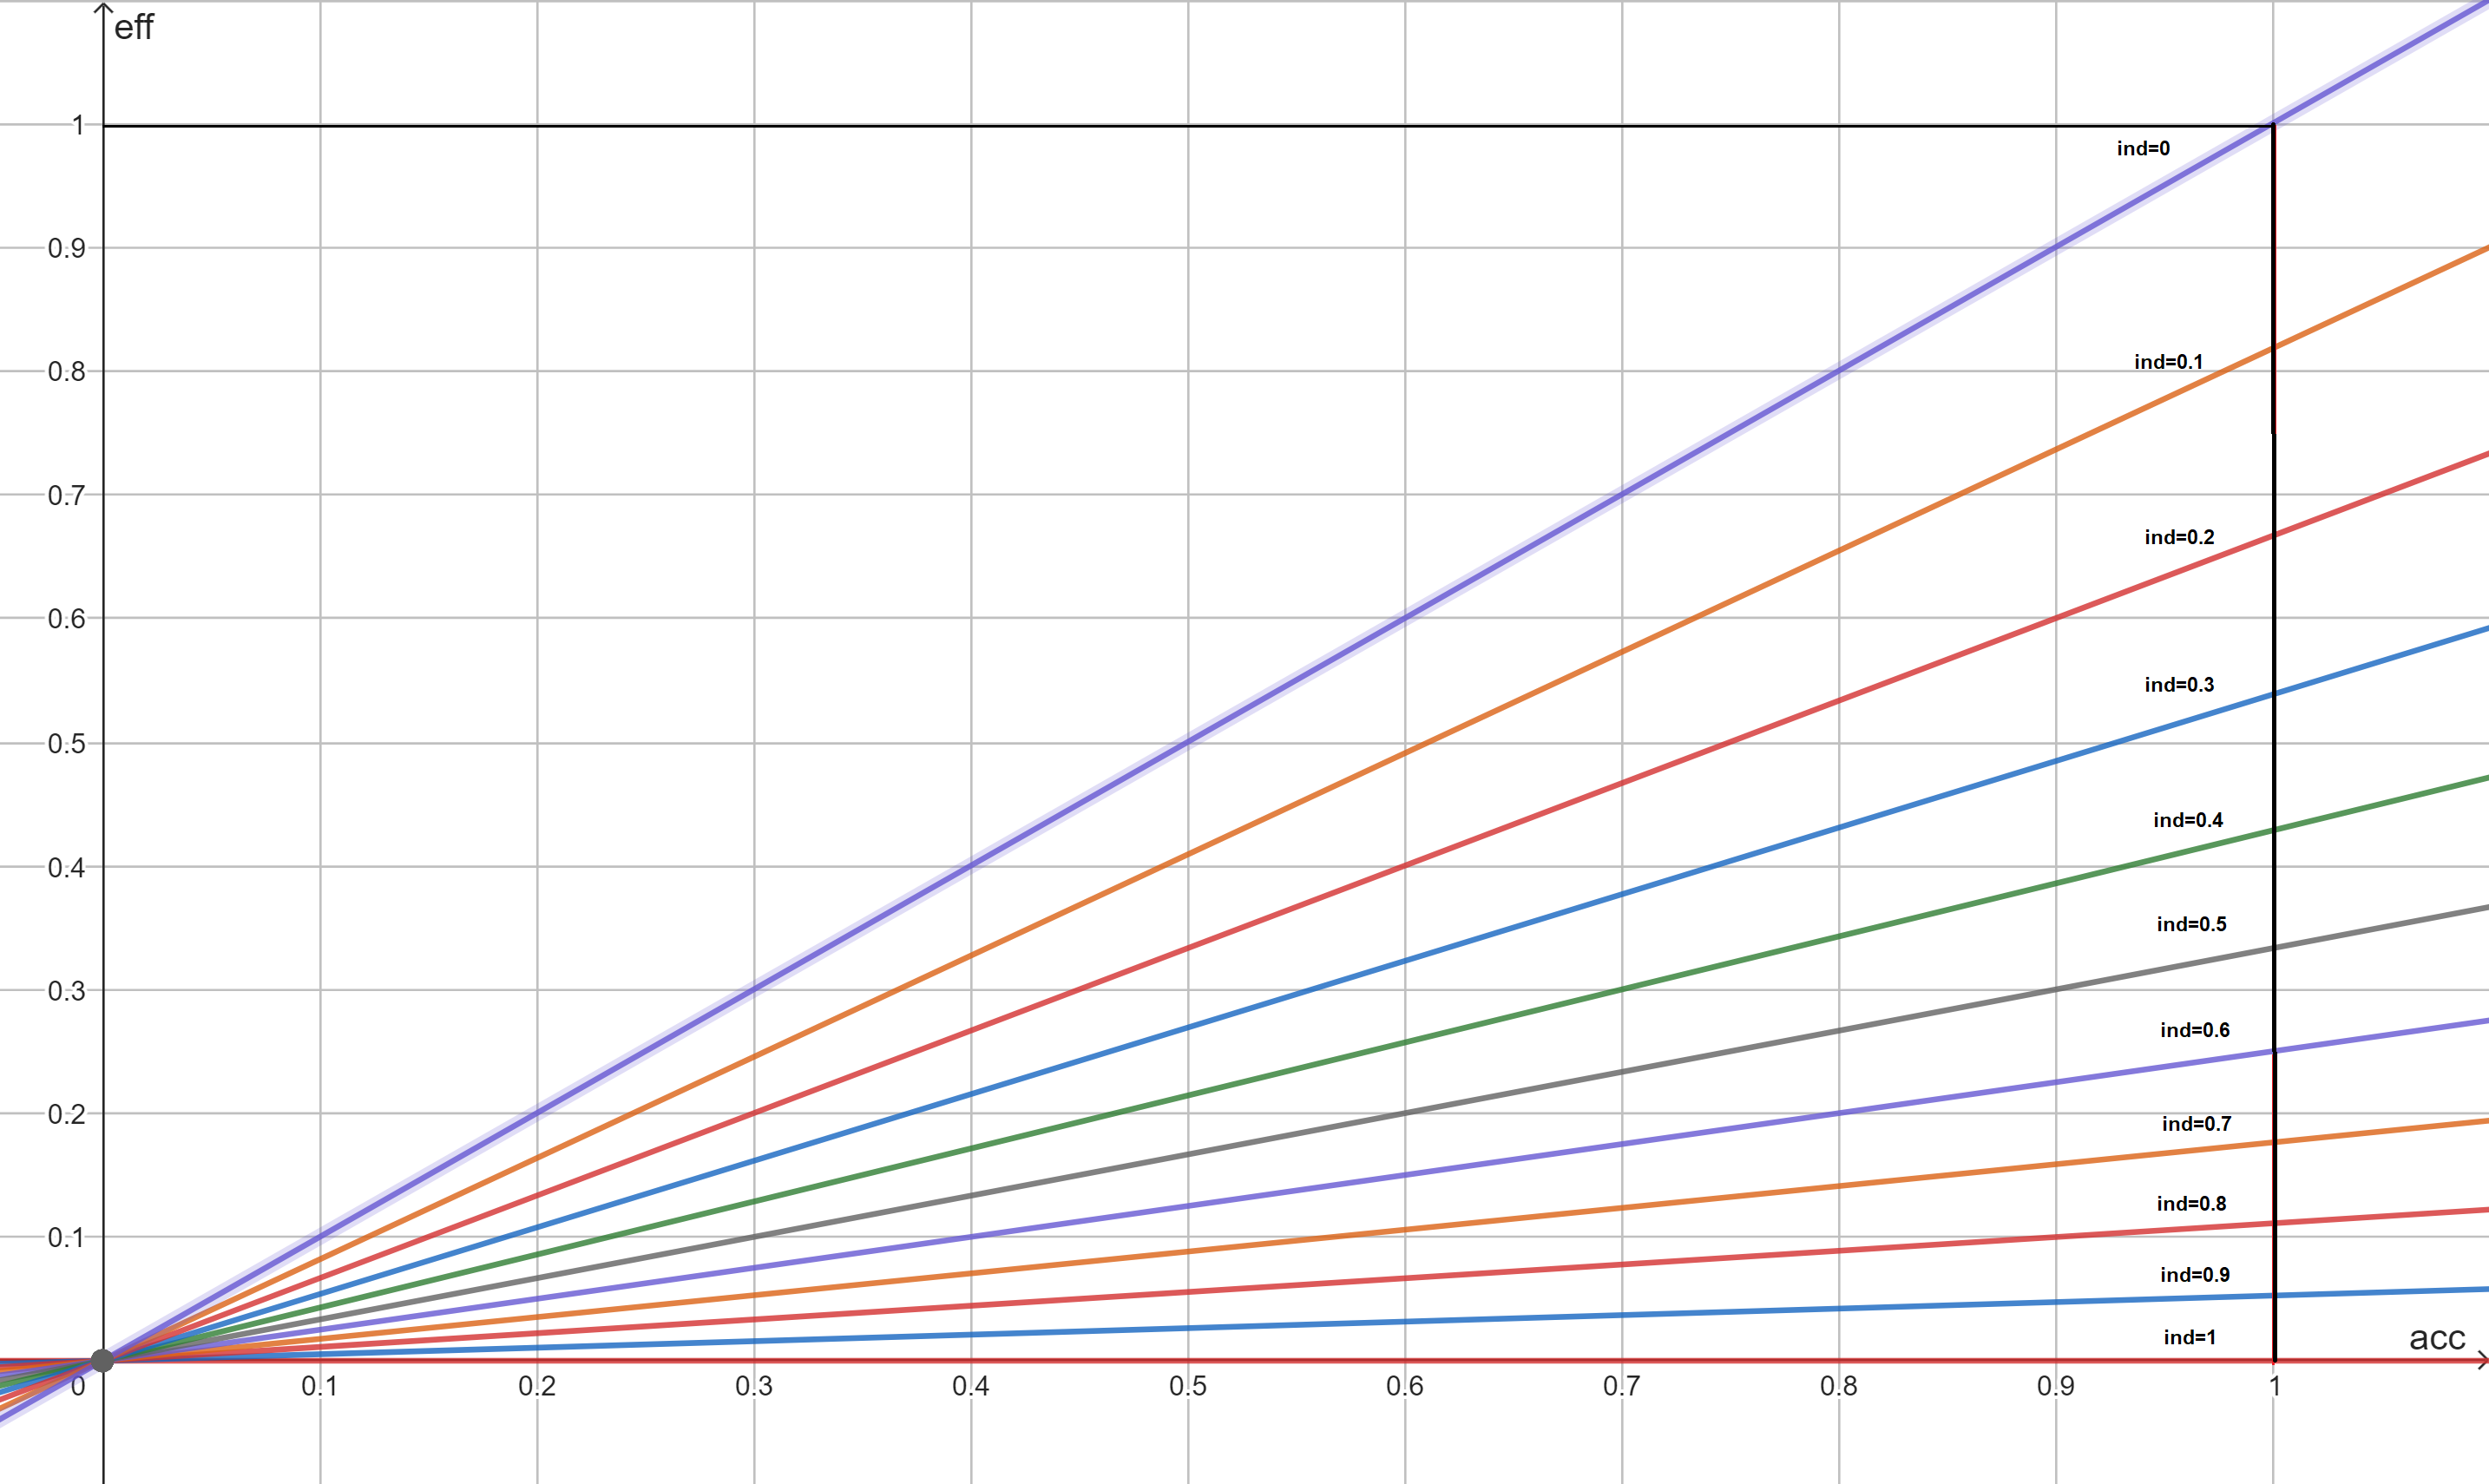
\includegraphics[width=0.9\linewidth]{ImageFiles/BNNRob/eff_vs_acc}
		\caption{Effectiveness trend with when the unknown ratio is fixed}
		\label{fig:eff_vs_acc}
	\end{subfigure}%
	\begin{subfigure}{.5\textwidth}
		\centering
		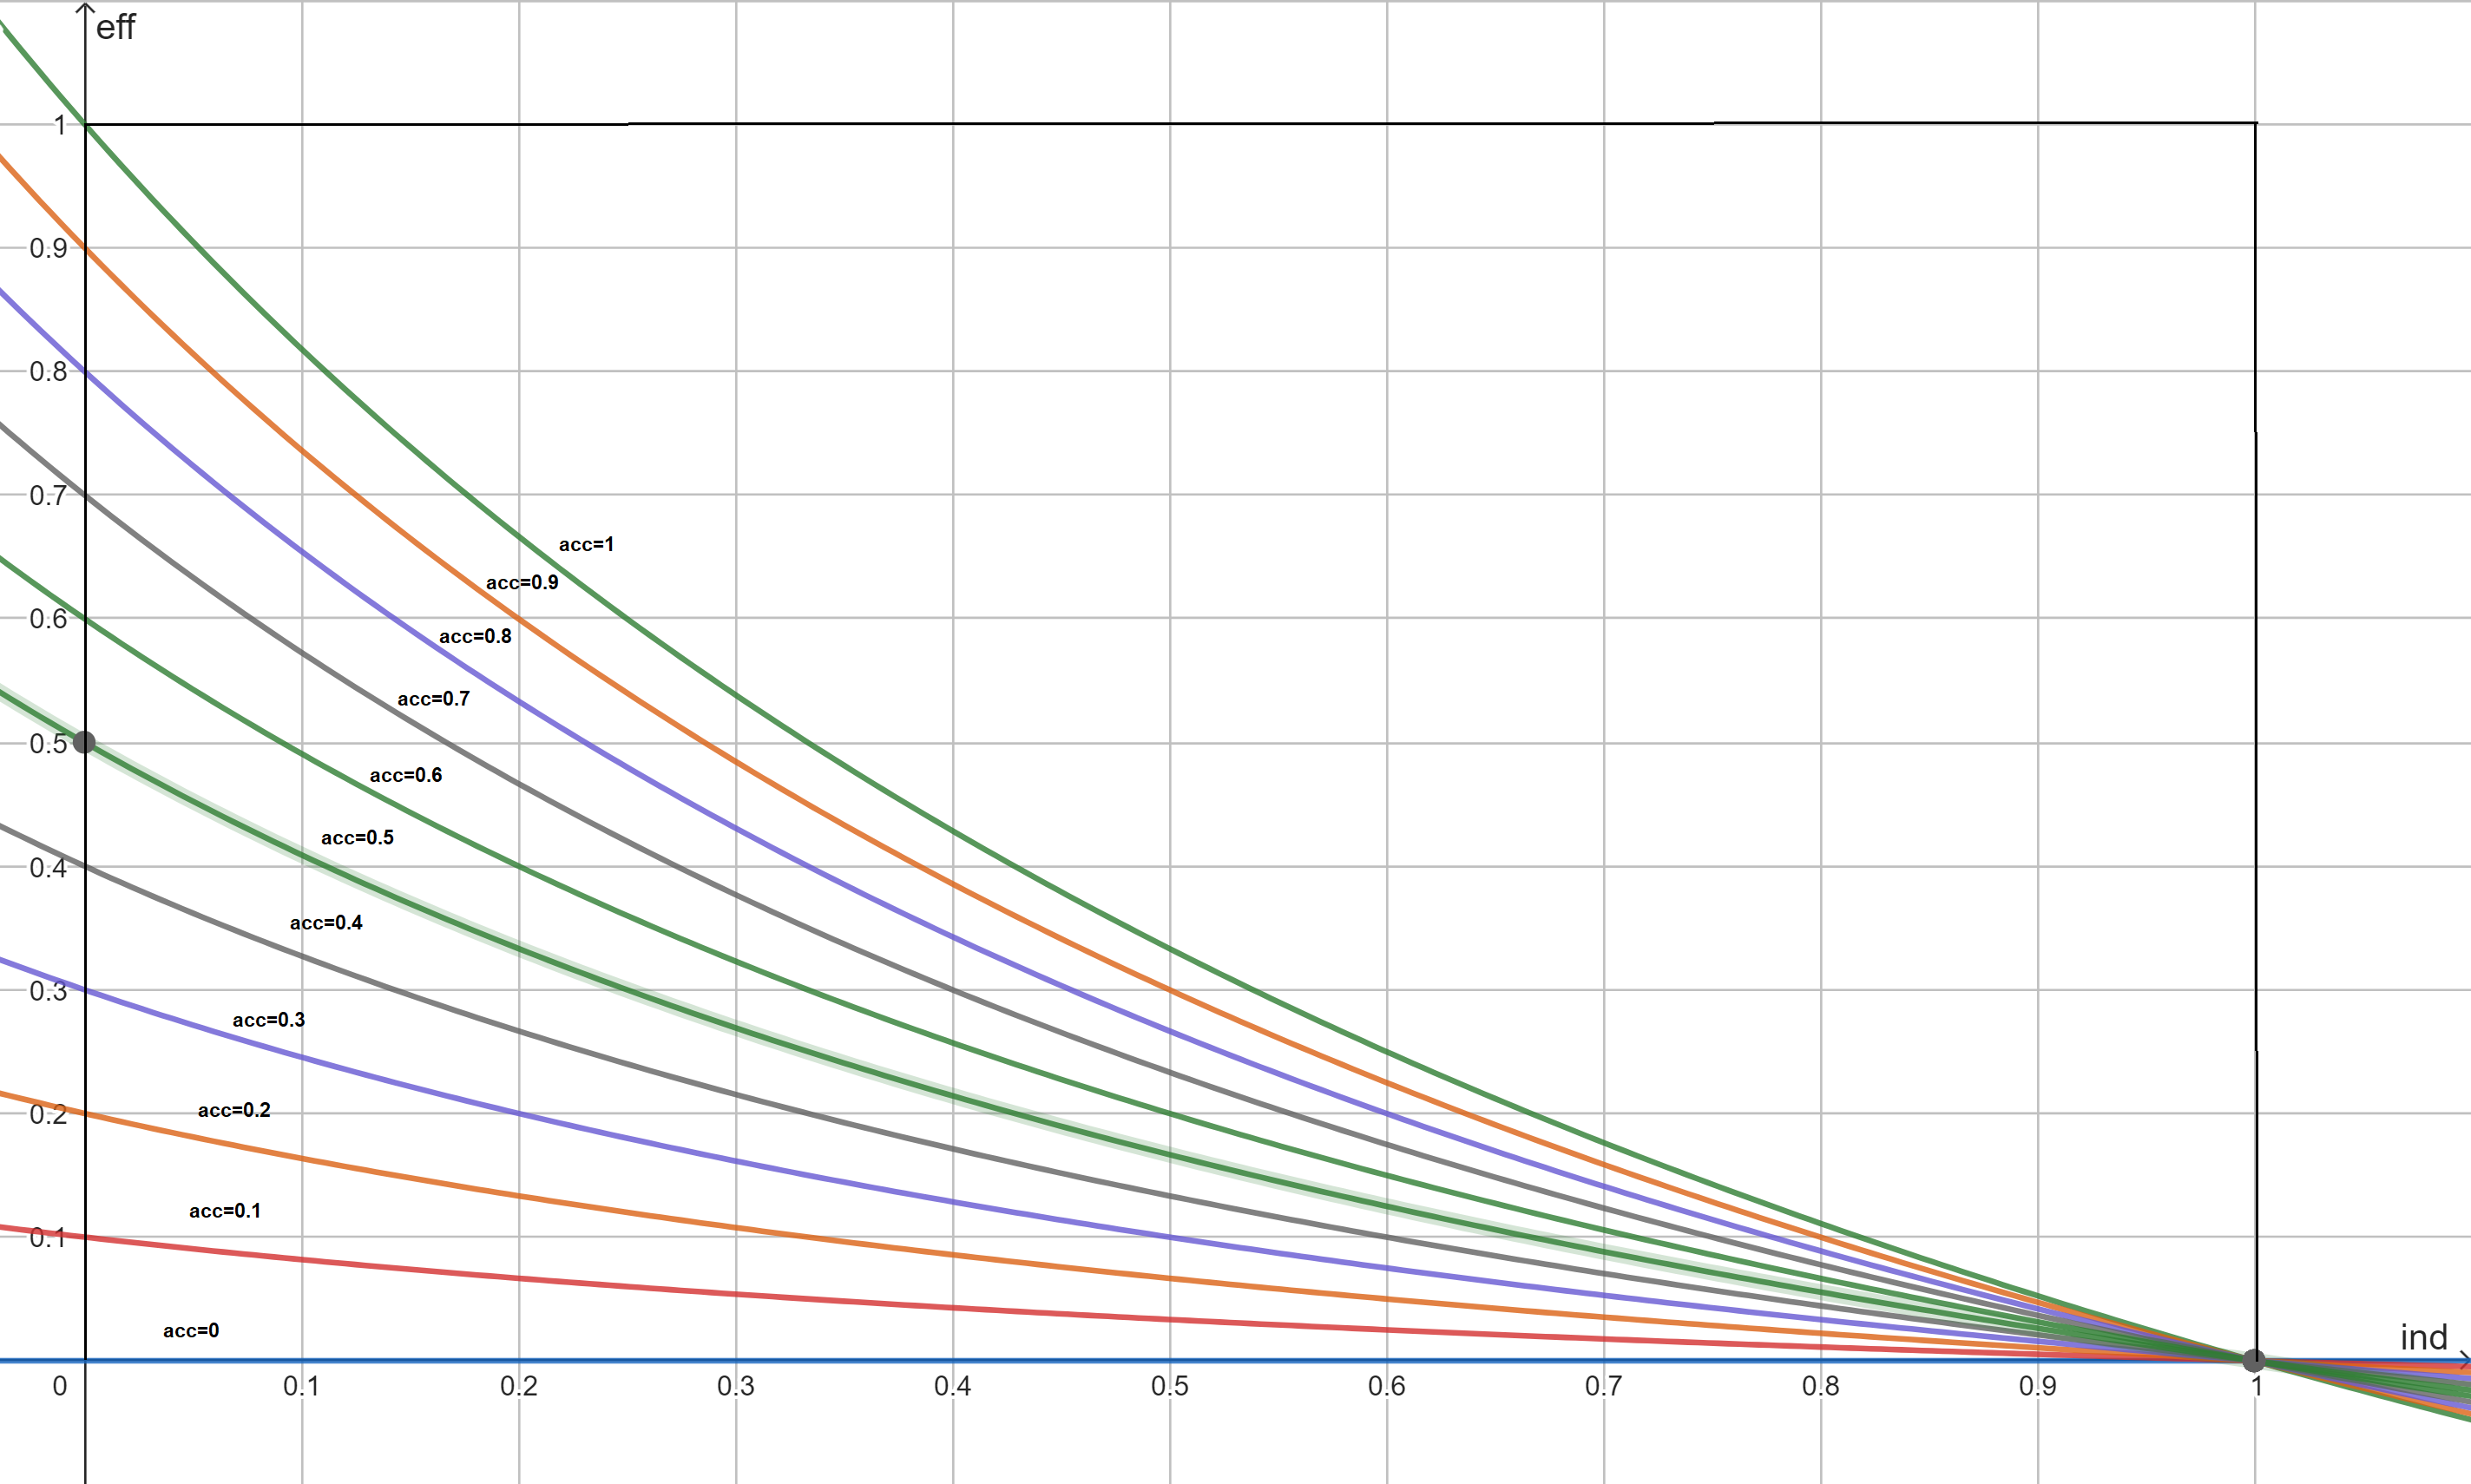
\includegraphics[width=0.9\linewidth]{ImageFiles/BNNRob/eff_vs_ind}
		\caption{Effectiveness trend with when the accuracy is fixed}
		\label{fig:eff_vs_ind}
	\end{subfigure}
	\caption{Effectiveness trend}
	\label{fig:eff_vs}
\end{figure}

The proposed measure can serve as a powerful tool for comparing and evaluating BNNs or any MLM that provides an uncertainty estimation. Its strength lies in the fact that it combines two different metrics into a single score, offering direct support in decision-making. However, for a comprehensive analysis, all three metrics should be considered, as each one can shed light on different aspects of the network under test.

With the introduction of this new measure, it is now possible to apply the robustness formula presented in \Def~\ref{def:rob3}, using the effectiveness instead of accuracy. The resulting metric would be an \textit{augmented} robustness, which takes into account both accuracy and network indecision, providing a more comprehensive assessment of model performance.

\begin{definition}\label{def:robaug} (Augmented robustness 3).
	Let $C$ be a classifier, $tol(x)$ a tolerance function and $dep(x)$ a penalization function.
	The augmented robustness $robAug_A(C,D) \in [0,1]$ of a classifier $C$ w.r.t. alteration of type A in the range $[L_A, U_A]$ on a dataset $D$ is defined formally as:
	\[
		robAug_A(C,D) = \frac{\int_{L_A}^{U_A} [tol(eff(C,D^{A_i}) - \beta) - dep(eff(C,D^{A_i}) - \beta)] \cdot p_A(i)\ di}{2} + \frac{1}{2}
	\]
	where $\beta$ is a threshold referring to minimum effectiveness accepted and $p_A$ is probability distribution of the alteration levels.
\end{definition}

In this definition, selecting an appropriate value for $\beta$ may not be as intuitive as in previous cases. One immediate choice could be to define $\beta = \frac{\Theta}{\gamma + 1}(1-\gamma)$, which is derived directly from the requirements on accuracy and unknown ratio. Although $\beta$ can be chosen in other ways, this choice provides a practical and intuitive starting point for its calculation.